可以从C++源码生成文档的成熟和流行的工具是Doxygen,其第一个版本是由Dimitri van Heesch在1997年10月发布的。从那时起,其存储库(\url{https://github.com/doxygen/doxygen})就得到了180多个贡献者的积极支持。

Doxygen可以生成以下格式的文档:

\begin{itemize}
\item 
超文本标记语言(HTML)

\item 
富文本格式(RTF)

\item 
便携式文件格式(PDF)

\item 
Lamport's TeX (LaTeX)

\item 
PostScript (PS)

\item 
Unix手册(man pages)

\item 
Microsoft课编译HTML帮助(CHM)
\end{itemize}

若用Doxygen指定的格式提供额外信息的注释装饰代码,其将解析为丰富的输出文件,还可以分析代码结构以生成有用的图表。后者是可选的,并且需要Graphviz工具(\url{https://graphviz.org/})支持。

开发人员首先应该回答以下问题:项目的用户是直接获得文档,还是自己生成文档(也许是在从源码构建时)?第一个选项意味着文档是随二进制文件一起提供的,可以在线获得,或者(不那么优雅地)与源代码一起存入存储库。

答案很重要,因为若希望用户在构建过程中生成文档,他们将需要系统中存在的依赖项。这不是一个太大的问题,因为Doxygen可以通过大多数包管理器(以及Graphviz)获得,所有需要的只是一个简单的命令,例如Debian的这个命令:

\begin{tcblisting}{commandshell={}}
apt-get install doxygen graphviz
\end{tcblisting}

Windows上也有可用的二进制文件(查看该项目的网站)。

为用户生成文档,或在需要时处理添加依赖项。这已经在第7章介绍过了,这里就不再赘述了。Doxygen是用CMake构建的,也可以使用源码生成。

在系统中安装Doxygen和Graphviz后,可以将生成添加到项目中。与网上消息来源不同,这并不像我们想象的那么困难或复杂。不需要创建外部配置文件,提供到doxygen可执行文件的路径,或添加自定义目标。从CMake 3.9开始,可以使用FindDoxygen查找模块中的doxygen\_add\_docs()函数,设置文档目标。

其签名是这样的:

\begin{lstlisting}[style=styleCMake]
doxygen_add_docs(targetName [sourceFilesOrDirs...]
	[ALL] [USE_STAMP_FILE] [WORKING_DIRECTORY dir]
	[COMMENT comment])
\end{lstlisting}

第一个参数指定目标名称,需要用-t参数显式地构建cmake(在生成构建树之后):

\begin{tcblisting}{commandshell={}}
cmake --build <build-tree> -t targetName
\end{tcblisting}

或者,可以通过添加ALL参数来构建(通常没有必要)。其他选项都是不言自明的,除了USE\_STAMP\_FILE。这允许CMake在没有任何源文件更改的情况下跳过文档的重新生成(但要求sourceFilesOrDirs只包含文件)。

我们将遵循前几章的实践,创建一个带有辅助函数的程序模块(可以在其他项目中重用):

\begin{lstlisting}[style=styleCMake]
# chapter-10/01-doxygen/cmake/Doxygen.cmake

function(Doxygen input output)
	find_package(Doxygen)
	if (NOT DOXYGEN_FOUND)
		add_custom_target(doxygen COMMAND false
			COMMENT "Doxygen not found")
		return()
	endif()
	set(DOXYGEN_GENERATE_HTML YES)
	set(DOXYGEN_HTML_OUTPUT
		${PROJECT_BINARY_DIR}/${output})
		
	doxygen_add_docs(doxygen
		${PROJECT_SOURCE_DIR}/${input}
		COMMENT "Generate HTML documentation"
	)
endfunction()
\end{lstlisting}

该函数接受两个参数——输入和输出目录——并将创建一个自定义doxygen目标:

\begin{enumerate}
\item 
首先,使用CMake的内置Doxygen查找模块来确定系统中是否有Doxygen可用。

\item 
若不可用,将创建一个伪doxygen目标,通知用户并运行一个错误命令,该命令(在类Unix系统上)返回1,导致构建失败。这时用return()结束函数。

\item 
若Doxygen可用,将在提供的输出目录中生成HTML。Doxygen是可配置的(在官方文档中找到更多信息),要设置任何选项,只需按照示例调用set()并在其名称前加上DOXYGEN\_。

\item 
设置实际的doxygen目标:所有DOXYGEN\_变量将转发到doxygen的配置文件中,文档将从源树中提供的输入目录生成。
\end{enumerate}

若文档是由用户生成的,步骤2可能需要安装必要的依赖项。

要使用这个函数,可以将其添加到项目的主列表文件中:

\begin{lstlisting}[style=styleCMake]
# chapter-10/01-doxygen/CMakeLists.txt

cmake_minimum_required(VERSION 3.20.0)
project(Doxygen CXX)
enable_testing()
list(APPEND CMAKE_MODULE_PATH "${CMAKE_SOURCE_DIR}/cmake")
add_subdirectory(src bin)

include(Doxygen)
Doxygen(src docs)
\end{lstlisting}

构建doxygen目标生成如下HTML文档:

\begin{center}
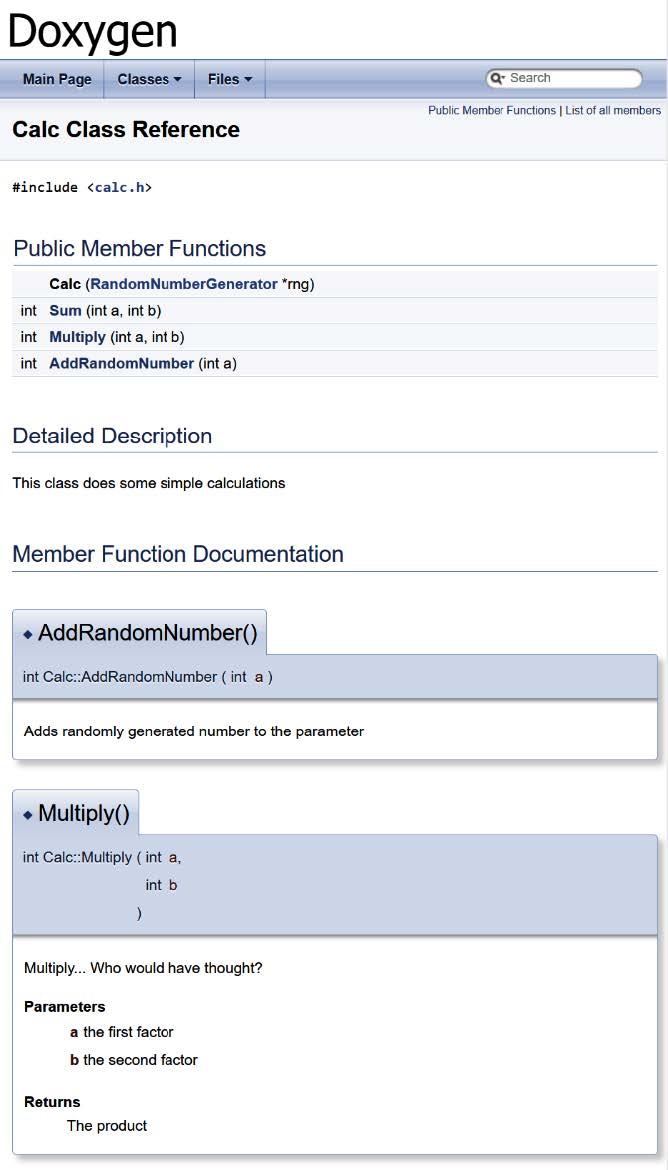
\includegraphics[width=0.8\textwidth]{content/3/chapter10/images/1.jpg}\\
图10.1 Doxygen生成的类引用
\end{center}

成员函数文档中可以看到,通过在头文件中用适当的注释在方法前面添加:

\begin{lstlisting}[style=styleCXX]
// chapter-10/01-doxygen/src/calc.h (fragment)

/**
Multiply... Who would have thought?
@param a the first factor
@param b the second factor
@result The product
*/
int Multiply(int a, int b);
\end{lstlisting}

这种格式称为Javadoc。打开带有双星号的注释块很重要:/**。更多信息可以在Doxygen的文档块描述中找到(参见扩展阅读部分的链接)。

若安装了Graphviz,Doxygen将检测它并生成依赖关系图:

\begin{center}
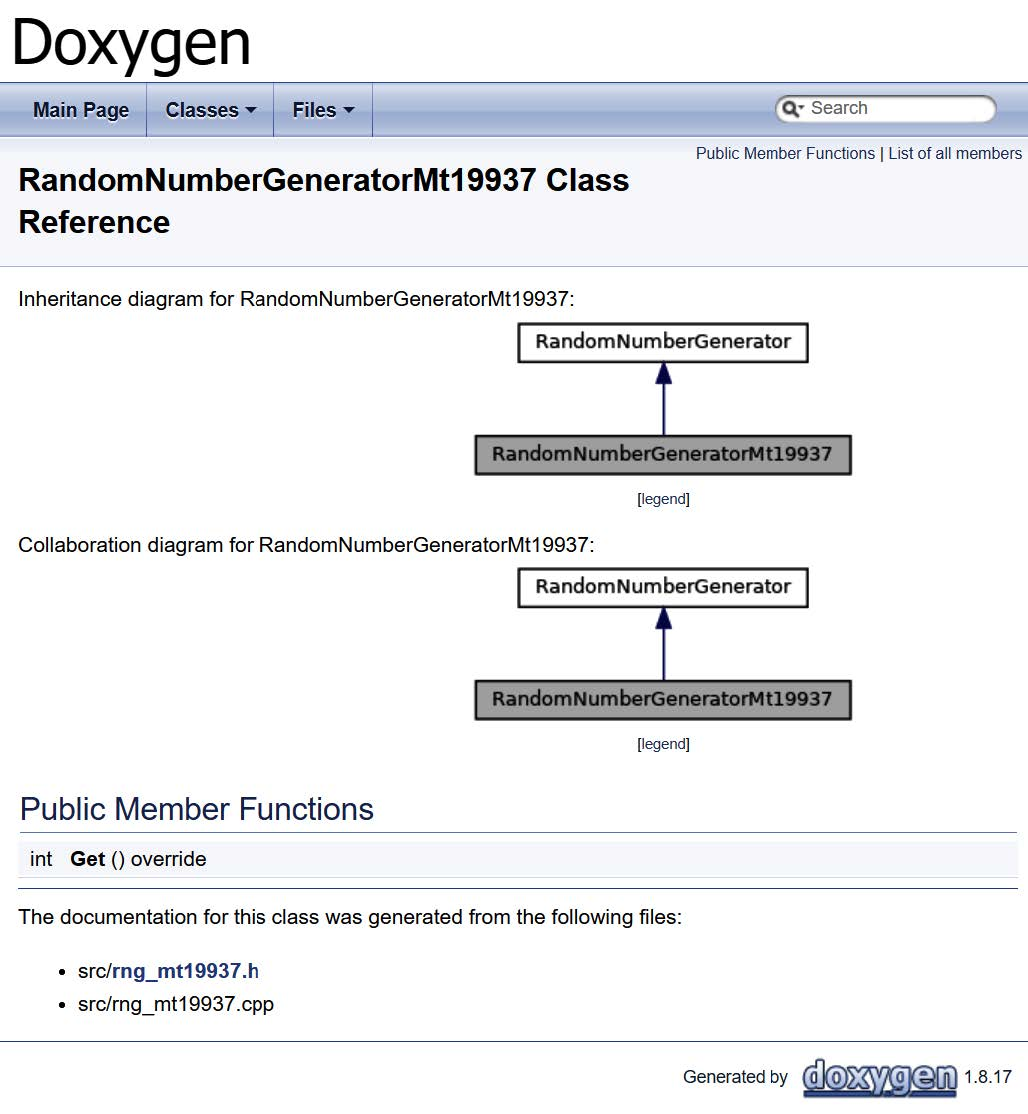
\includegraphics[width=0.8\textwidth]{content/3/chapter10/images/2.jpg}\\
图10.2 Doxygen生成的继承和协作图
\end{center}

通过直接从源代码生成文档,创建了一种机制,可以使用整个开发周期中发生的更改快速更新文档。此外,注释中的遗漏都有可能在代码审查期间发现。

许多开发者会抱怨Doxygen提供的设计过时了,这让他们在向客户展示生成的文档时犹豫不决。别担心,这个问题很容易解决。









